\chapter{Effects of localised shearing on crystal growth and nucleation}
As outlined in Chapter 1, the original outline of the PhD was to investigate the possibility of using optical tweezing as a means of initiating and controlling nucleation by generating fluid flow within a small droplet of supersaturated solution. The goal of which would be to allow the understand the influence of shearing on nucleation at a micro level as compared to larger scale results. It has been shown that for macro-scale systems, the likelihood of nucleation increases to a maximum value under increased shearing \cite{Debuysschere2023, Mura2016}. Theoretical research into the matter identified two competing effects that effect a crystal in moving fluid fields; firstly, nucleation is enhanced due to the increased mass transfer of solute material; and secondly, shear flow against the crystal surface leading to a decrease in growth \cite{Mura2016}. These two competing effects are validated by experimental work using glycine solutions, showing that beyond a certain shear rate the nucleation rate is reduced \cite{Debuysschere2023}. In this chapter I outline the optical tweezer equipment used during this PhD, the initial attempts made to induce nucleation via optical rotation, and the impact of a moving beam on the crystal growth of a newly formed nucleus. 

\section{Optical Tweezer Equipment}
In general, all optical tweezers require a laser driver, two
microscope objectives (one for trapping and one for imaging),
and a means of controlling the position of the loaded sample. 
While there are other pieces of equipment used in modern tweezer
experiments these are the bare minimum requirements for any 
optical tweezer. The laser used for this project was a 1064 
nm near infrared laser - provided by CNI Lasers – that has 
an adjustable power supply to vary the energy output of the 
laser - the remaining optics where supplied by Thor Labs.
Experimental work has shown that the trapping efficiency 
increases with beam diameter up until it exceeds $\frac{2}{3}D_{obj}$ 
\cite{kim2003dependence} where $D_{obj}$ is the diameter
of the objective aperture. To expand the beam front we 
utilise a Galilean beam expansion arrangement (indicated 
by $f_1$, and $f_2$) as recommended for high power laser 
applications. In our initial experiments the beam expansion 
provides a $4\times$ magnification; however, in later experiments 
where we utilise a galvano-mirror the beam expansion is $3\times$ 
and then the 4f correlator provides a further $1.25\times$ magnification 
(using $f_3$ and $f_4$) - where the magnification is given by.
\begin{align}
	\frac{D_2}{D_1} = \frac{f_2}{f_1}
\end{align}
It should be noted that the galvano-mirror requires the use 
of a Keplerian beam expansion arrangement which reduces
the transmitted laser power due to localised heating of the air.
Afterwards the laser is passed through a dichroic mirror that 
separates incoming infrared and visible light, this is to 
prevent the laser from damaging the CCD camera used for imaging
the trapping plane. The laser is then focused to a diffraction
limited spot by a 1.25 NA objective. By increasing the numerical
aperture of the objective, the gradient force at the focal point 
is increased; the trade-off being that the for higher NA values 
the trapping depth is reduced due to spherical aberrations.
While it is possible to increase the trapping depth \cite{Reihani2006} 
by adjusting the objective's tube length this approach is incompatible 
with our trapping arrangement. A 0.25 NA condenser objective refocuses
the scattered laser light and also provide an aperture for an 
imaging LED to illuminate the focal plane. Samples are loaded 
onto a piezo driven table to that is inserted between the trapping
and condensing objectives; the piezo drivers allow for sub-micron
control of the sample position to a degree as small as a 10 nm. 
To detect and monitor the position of a trapped particle a 
quadrant photo diode (QPD) was utilised. 

\begin{figure}
	\label{fig:setup}
	\centering
	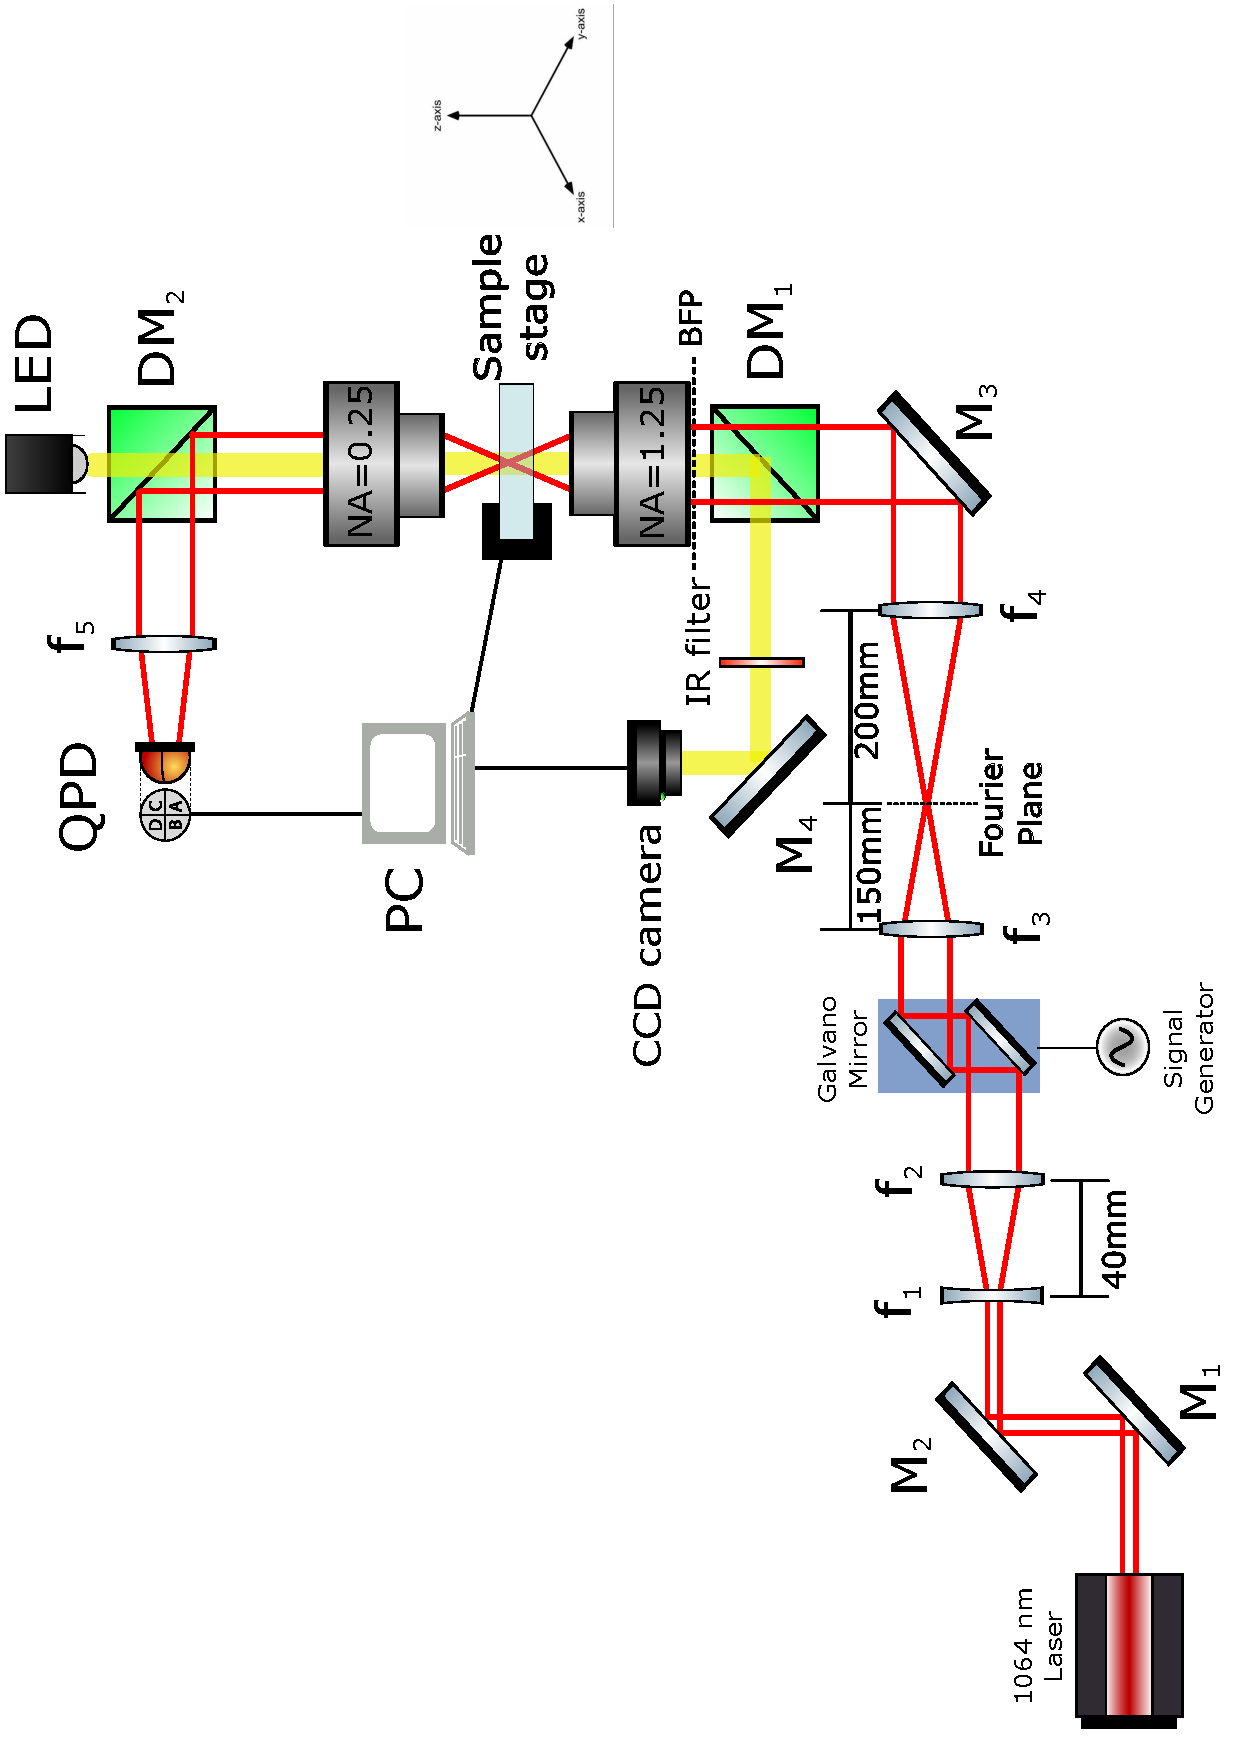
\includegraphics[height=\linewidth, angle=270]{tweezer_setup.pdf}
	\caption{Optical tweezer set up used for the majority of the PhD. The focal lengths of $f_1$, $f_2$, $f_3$, \& $f_4$ are $-20\ mm$, $60\ mm$, $150\ mm$, \& $200\ mm$ respectively. Diagram not drawn to scale.}
\end{figure}

\subsection{Position detection methods}
In order to accurately capture the dynamics of a trapped particle, 
a position detection system must be utilised. There are 3 possible
methods of position detection: video-analysis, lateral-effect
position sensing, and quadrant photodiodes. The former being 
ideally suited for multiple traps or situations where precision
is not the top priority. In order to match the force measurements
of back-focal plane interferometry requires the camera's frame
rate to exceed $1\ kHz$ which can be difficult to achieve while 
maintaining a decent resolution \cite{Gibson2008}. In comparison
off the shelf back-focal plane detectors can achieve temporal
resolutions anywhere from $10-100\ kHz$. 
 
A QPD is frequently used position detection system for optical 
tweezers due to their high sampling rate, high degree of 
precision, and ease of set up. The QPD is constructed of four photo 
diodes assembled in a quadrant formation, when a particle is trapped the 
interference pattern produced is focused onto the QPD, with 
the maximum intensity mapping to the particle's centre of mass. 
By summing the voltages of the horizontal and vertical quadrants 
together the particle's centre of mass is tracked in the x-y 
plane. Axial displacement can be estimated by observing the change
in the total voltage of the QPD. The outputted signal gives an
indication of the particle's relative displacement from the beam 
focus, but in order to convert the signal to distance units the
trap needs to be calibrated (assuming a linear response curve).

\begin{figure}[h!]
	\centering
	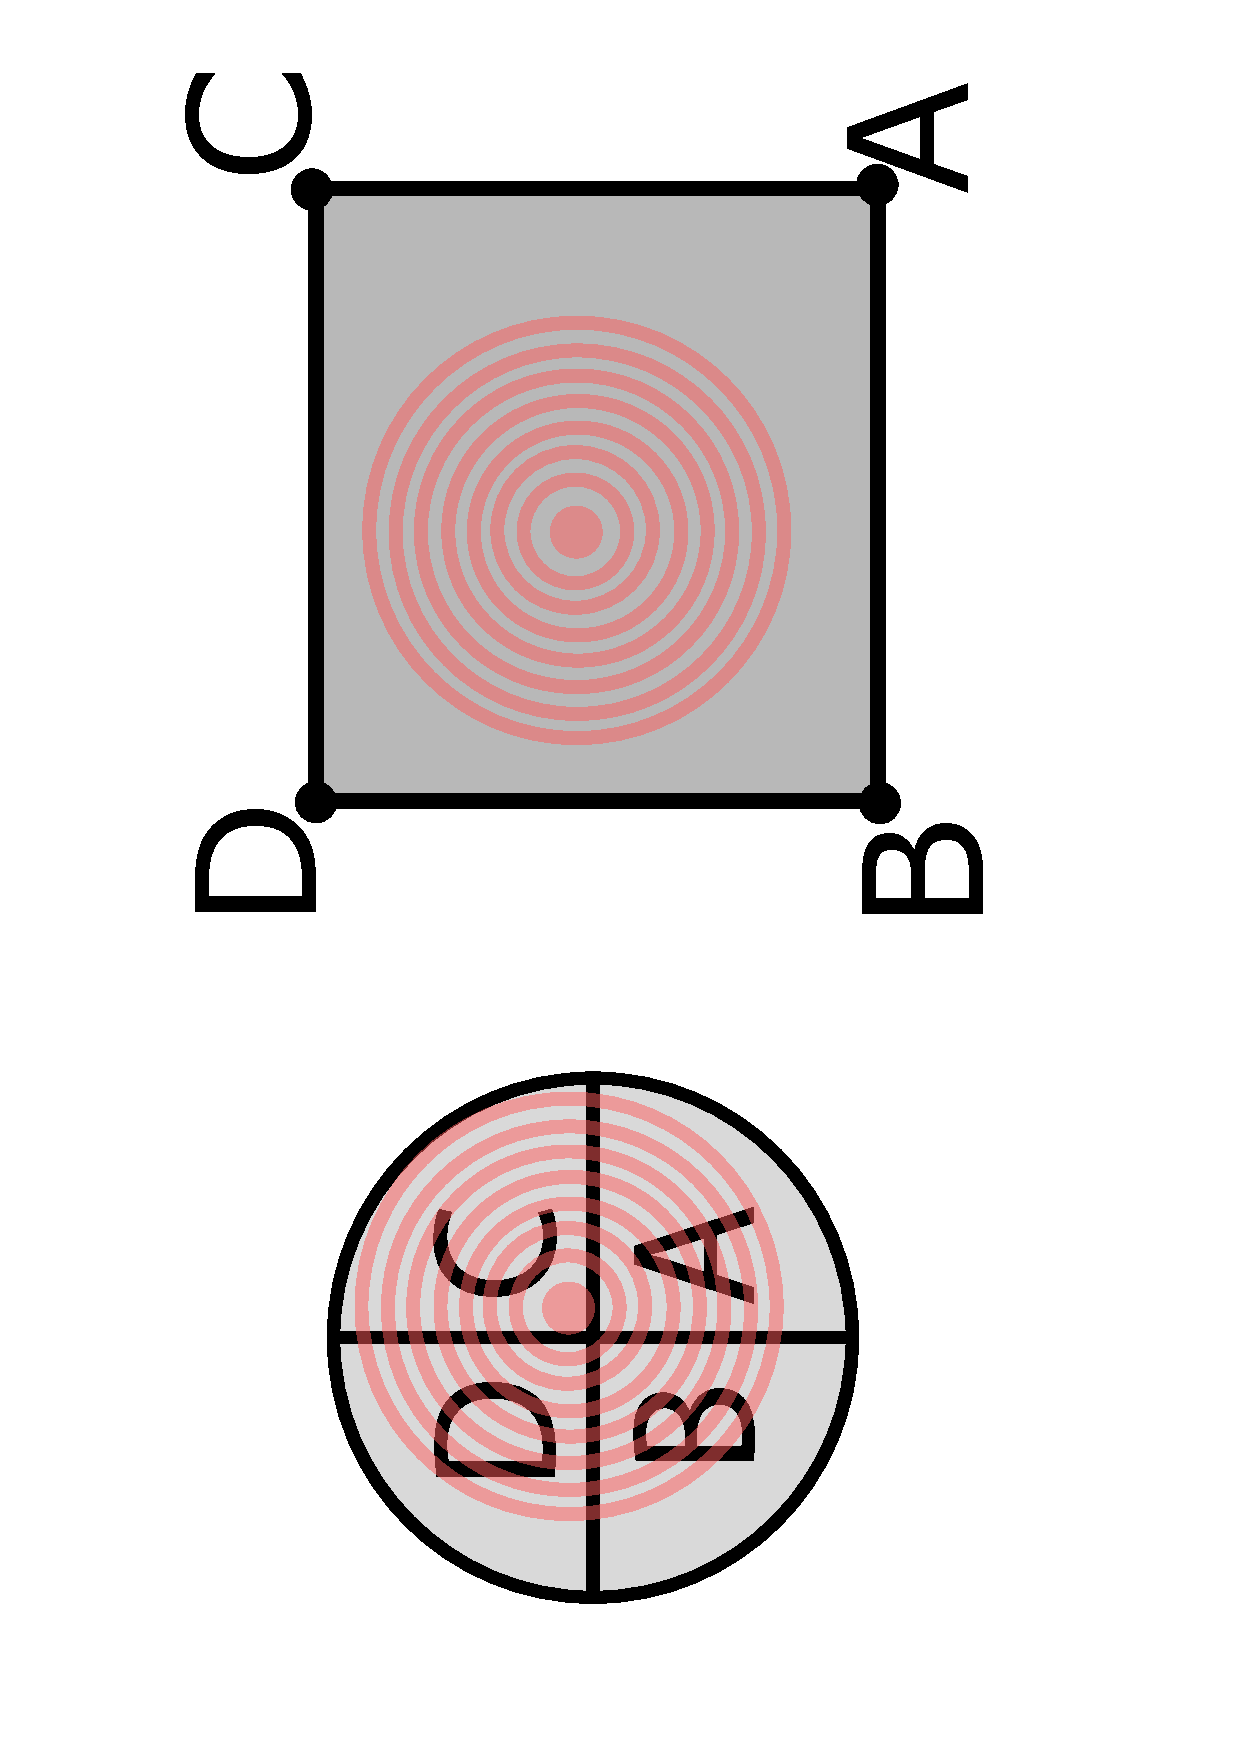
\includegraphics[height=\linewidth, angle=270]{QPD_Lateral_effect.pdf}
	\caption{Comparison between QPD and Lateral effect photodiodes.
	The four quadrants of a QPD (left) experience different photocurrents
	based on the total intensity of light incident on each section 
	(labelled A, B, C, D). 
	Whereas a Lateral effect sensor (right) uses the resistive properties
	of the photodiode surface to vary the create different photocurrents 
	passing through the anodes A, B, C, and D.}
\end{figure}

A lateral-effect sensor has a similar output but works using a 
the entire sensor as a single cell analogous to the focal plane of
the trapping beam. The four corners of the sensor act as anodes 
connected to a base plate cathode, as the beam moves across the
surface of the detector each anode will experience a different 
photocurrent depending on how close the centre of the 
interference pattern is to each anode. The advantage of a 
lateral effect detector is that the linear regime is much larger 
than a QPD making it much better for monitoring the position of a
trapped particle. However, Lateral-effect sensors are often limited
in their spacial resolution due to high signal-to-noise ratios, 
requiring a high intensity of light on the sensor in order to 
get a clean signal. As a result, most optical trapping experiments
are conducted using a QPD as opposed to a lateral-effect sensor, 
as often the displacement is small enough that the QPD response 
curve can be considered linear.

\section{Calibration of Tweezer Setup}
Prior to testing optical rotation the trapping laser was calibrated 
using power spectra analysis


\section{Synthesis of Birefringent Micro spheres}
\label{sec:vaterite}
Generation of fluid shear can be achieved via two avenues: Firstly, by 
utilising circularly polarised light it is possible to transfer angular 
momentum from the laser to the trapped entity. Secondly, one can 
directly move the trap within the imaging plane by steering the beam 
using either a galvanometric mirror or gimbal mirror. The following 
chapter outlines the work done with shear generated by circularly 
polarised light and the challenges of applying this to localising 
nucleation. 

There are several options for particles that can be rotated using 
optical tweezers \cite{Parkin2009, Saito2022}. Over the course of 
the PhD two different micro 
spheres where investigated, vaterite and liquid crystal droplets. Both 
can be readily synthesised in the lab and are will rotate at a variety 
of sizes. While silver nano particles were considered their high cost 
and small size meant they were disregarded as an option for optical 
rotation. 

Vaterite samples where made by the first preparing equal amounts of 
$CaCl_2$ and $NaCO_3$ at a concentration of $0.1M$, at the same time
a vial of $0.03M\ MgSO_4$ was prepared and set aside for later. First
a small vial was filled with $1.5mL$ of $CaCl_2$ followed by $60\mu L$ 
and $90\mu L$ of $MgSO_4$ and $NaCO_3$ respectively, forming a seed solution. 
Next, a larger vial was filled with $5\ mL$, $1.5\ mL$, and $1\ mL$ of
$CaCL_2$, $MgSO_4$, and $NaCO_3$ respectively followed by the seed solution. 
After 10 minutes of slow but continuous mixing a few drops of Agepon was added
to halt the reaction, the solution was filtered and washed 3 times with 
distilled water before being suspended in water. 

\subsection{Rotation of Vaterite micro spheres}
Vaterite is a polymorph of calcium carbonate that is rarely seen in 
nature due to its low stability. However unlike its other polymorphs of 
calcite and aragonite, when synthesised vaterite will typically form 
small spherical particles making them ideal for optical trapping. 
Synthesis of vaterite micro spheres requires fine control of the nucleation process in order to maintain polymorphic control. 

\section{Shear induced Nucleation}
\comment{This belongs in the introduction chapter me thinks}

It has long been known that solution nucleation is influenced by shearing of the fluid, from stirring agents in the container (i.e. propellers) to the container boundary layers, however there has yet to be a clear mechanism by which said shearing effects the nucleation event. Theoretical research into shear induced nucleation suggests that there should be a slight increase in the nucleation rate at low shear rates, reaching a maximum increase in nucleation rate, and then at higher shear rates the nucleation rate begins to drop off. This has been shown theoretically for both simple colloidal \cite{Mura2016,Debuysschere2023,Richard2015}  and ice crystal formation \cite{Goswami2020}; however, no experimental work into these systems has been conducted to prove this is the case.  There is some experimental evidence for this phenomena in simple salt and protein solutions - though the authors emphasise that mechanical agitation cannot be ruled out - there has not been a exhaustive study into the shearing effects apart from in glycine solutions. In \cite{Debuysschere2023} it was found that a shear rate of around $3000\ s^{-1}$ was the maximum shear rate that would yield the highest nucleation rate. Using the theoretical model established in \cite{Mura2016,2001} which modifies the CNT to account for the effects of a nucleus undergoing shearing, accounting for the fact that a nucleus' growth is undergoing competition between flow-mediated molecular transport and the strain applied by the flow field which inhibits the growth of the nucleus. There central conclusion (from both the theoretical and experimental results) is that there is an optimal shear rate in which the nucleation rate is maximised. However, a question that arises from this result, if there is a optimal shear rate in which molecular transport is maximised and strain is minimised, then surely there should also be a shear rate in which the molecular transport and strain are equal - allowing one to suspend a nucleus at a constant radius. In this scenario, the molecular transport would prevent the nucleus from dissolving, but the strain would prevent the nucleus from growing. This however would require one to be able to apply a continuous shear rate to a targeted nucleus with high precision, there is also no model for an individual nucleus undergoing growth. 

Optical tweezing has often been used for micro-rheology, by computing the
exact forces being exerted on the trapped sphere, one can determine the
local temperature/viscosity of the medium \cite{Millen2014, RodriguezSevilla2018}.
Typically one would use a birefringent particle (i.e. vaterite, liquid
crystals, etc) and rotating it within the fluid, the maximum rotation
rate being a product of the fluid drag resisting the torque of the 
trapping beam \cite{RodriguezSevilla2018}. Or if you want to measure 
fluid flow you can instead use a micro-rotor to see how fluid flow 
propagates in the medium \cite{Knoener2005}. Likewise, one can use 
a galvanometric mirror to probe the drag force of the fluid, by 
understanding the trap strength (calibrating using a low frequency 
signal) one can measure the drag force experienced by the local fluid \cite{RobertsonAnderson2018}. I

Understanding the fluid velocity around our trapped object is determined 
mostly by the Reynold's number of our system, for a sphere submersed 
in a moving fluid of velocity $U$ this is given by:
\begin{align}
	Re = \frac{\rho UD}{\mu}
\end{align}
Where $D$ is the sphere's diameter, and $\rho$ and $\mu$ are the fluid's density and viscosity respectively. In our case we do not have a fluid moving around a sphere but a sphere moving through the fluid at some velocity $U$, assuming a no-slip boundary condition we can model the fluid velocity profile based on the velocity of the particle. There are two possible avenues for generating shear flow with a trapped particle; rotation of birefringent particles, and fluid flow induced by particle motion. 

Rotating birefringent particles are by far the most common method for generating and measuring fluid flow in a solution. To see if we can even achieve the theoretical maximum shear rate, vaterite spheres were synthesised (see Sec.\ref{sec:vaterite}) submerged in water and trapped with the 1064 nm laser at set to 450 mW. The rotation frequency was determined using the QPD, and the particle sizes were computed by image analysis. With the particle size and rotation frequency, the tangential rotation speed is calculated via:
\begin{align}
	\label{eq:birefringent_speed}
	u(r) = \frac{\pi}{4}\frac{d^3}{r^2}\omega
\end{align}

Where $d$ is the particle diameter, $\omega$ is the rotation frequency
reported by the QPD, and $r$ is the distance from the particle's centre. 
Using Eq.\ref{eq:birefringent_speed} we computed the fluid flow radiating
outward from the centre of the sphere. The shear rate can then be computed
as the partial derivative fluid flow (assuming shearing is generated purely
by the flow field):
\begin{align}
	\label{eq:birefringent_shear}
	\dot{\gamma}(r)=\left|\frac{\delta u(r)}{\delta r} \right|= \frac{\pi}{2}\frac{d^3}{r^3}\omega
\end{align}

First we tested the rotational behaviour of vaterite in distilled water, 
samples of vaterite where diluted down and $200\mu L$ was pipetted onto
the sample stage. Due to Van der Waal's forces some of the microspheres 
were stuck together, fortunately individual sphere's were still

\begin{figure}[h!]
	\label{fig:vaterite_shear}
	\begin{subfigure}{0.5\linewidth}
		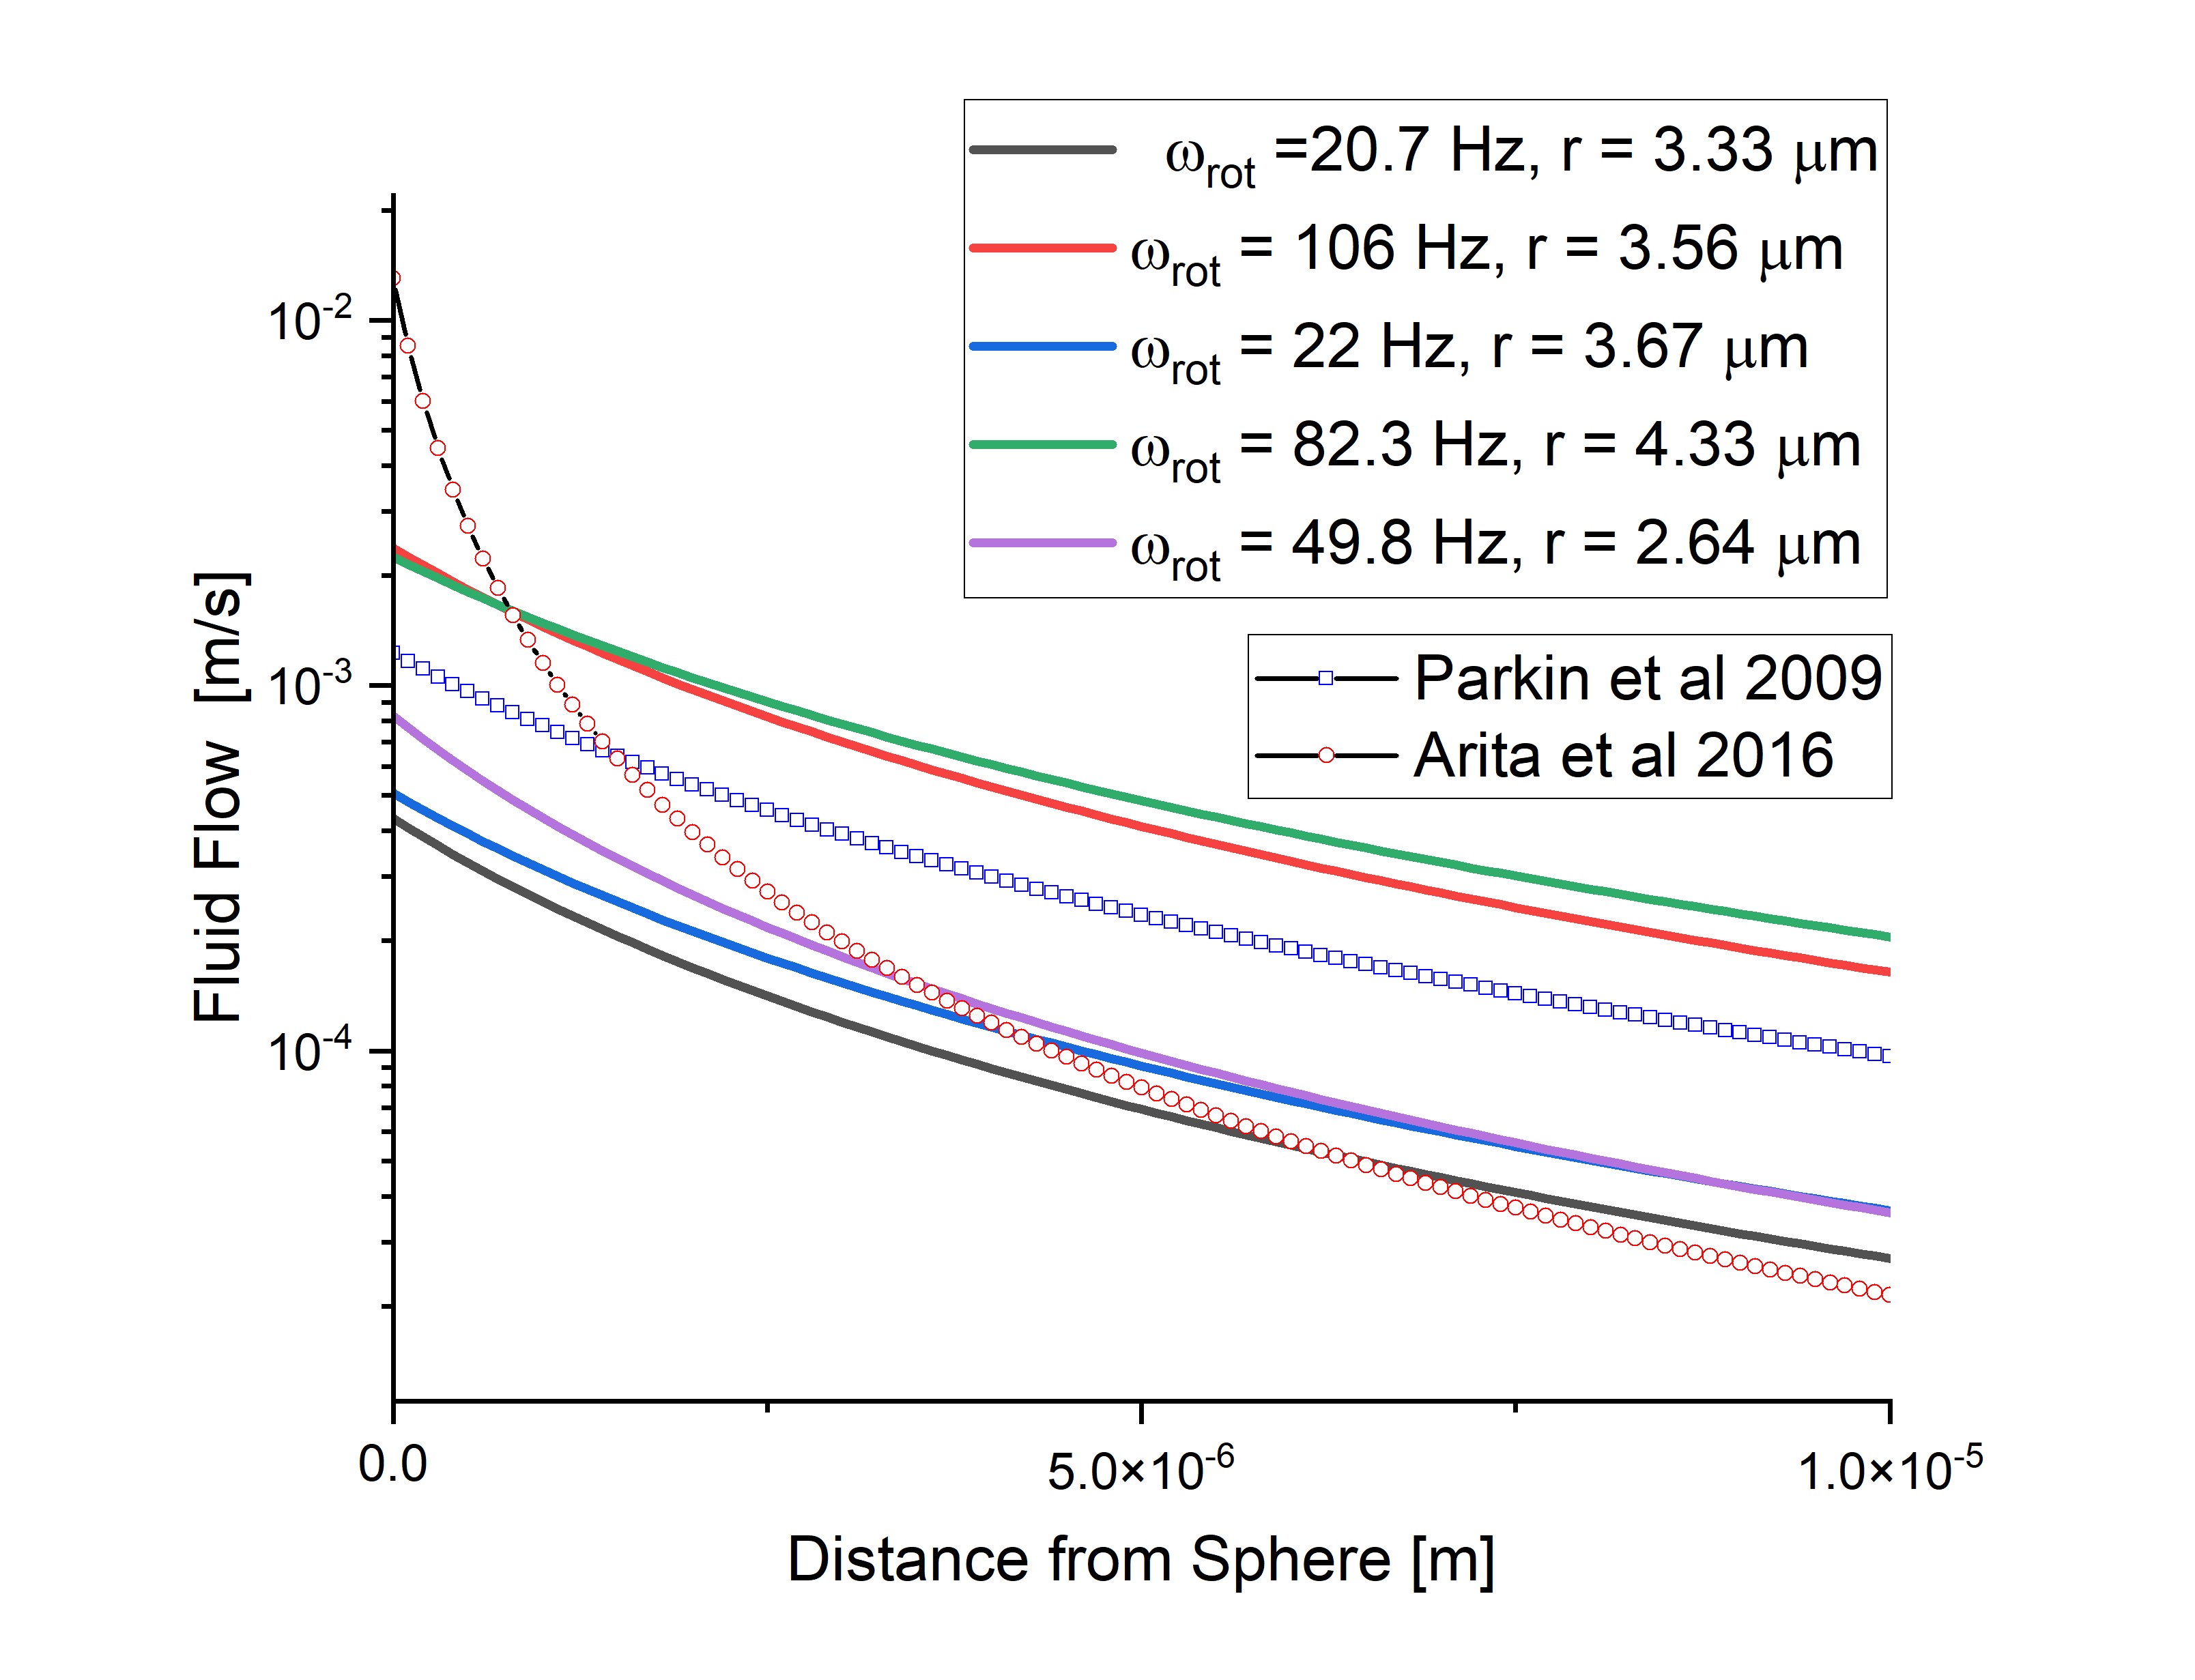
\includegraphics[width=\linewidth]{vaterite_fluid_flow.png}
		\subcaption{}
	\end{subfigure}
	\begin{subfigure}{0.5\linewidth}
		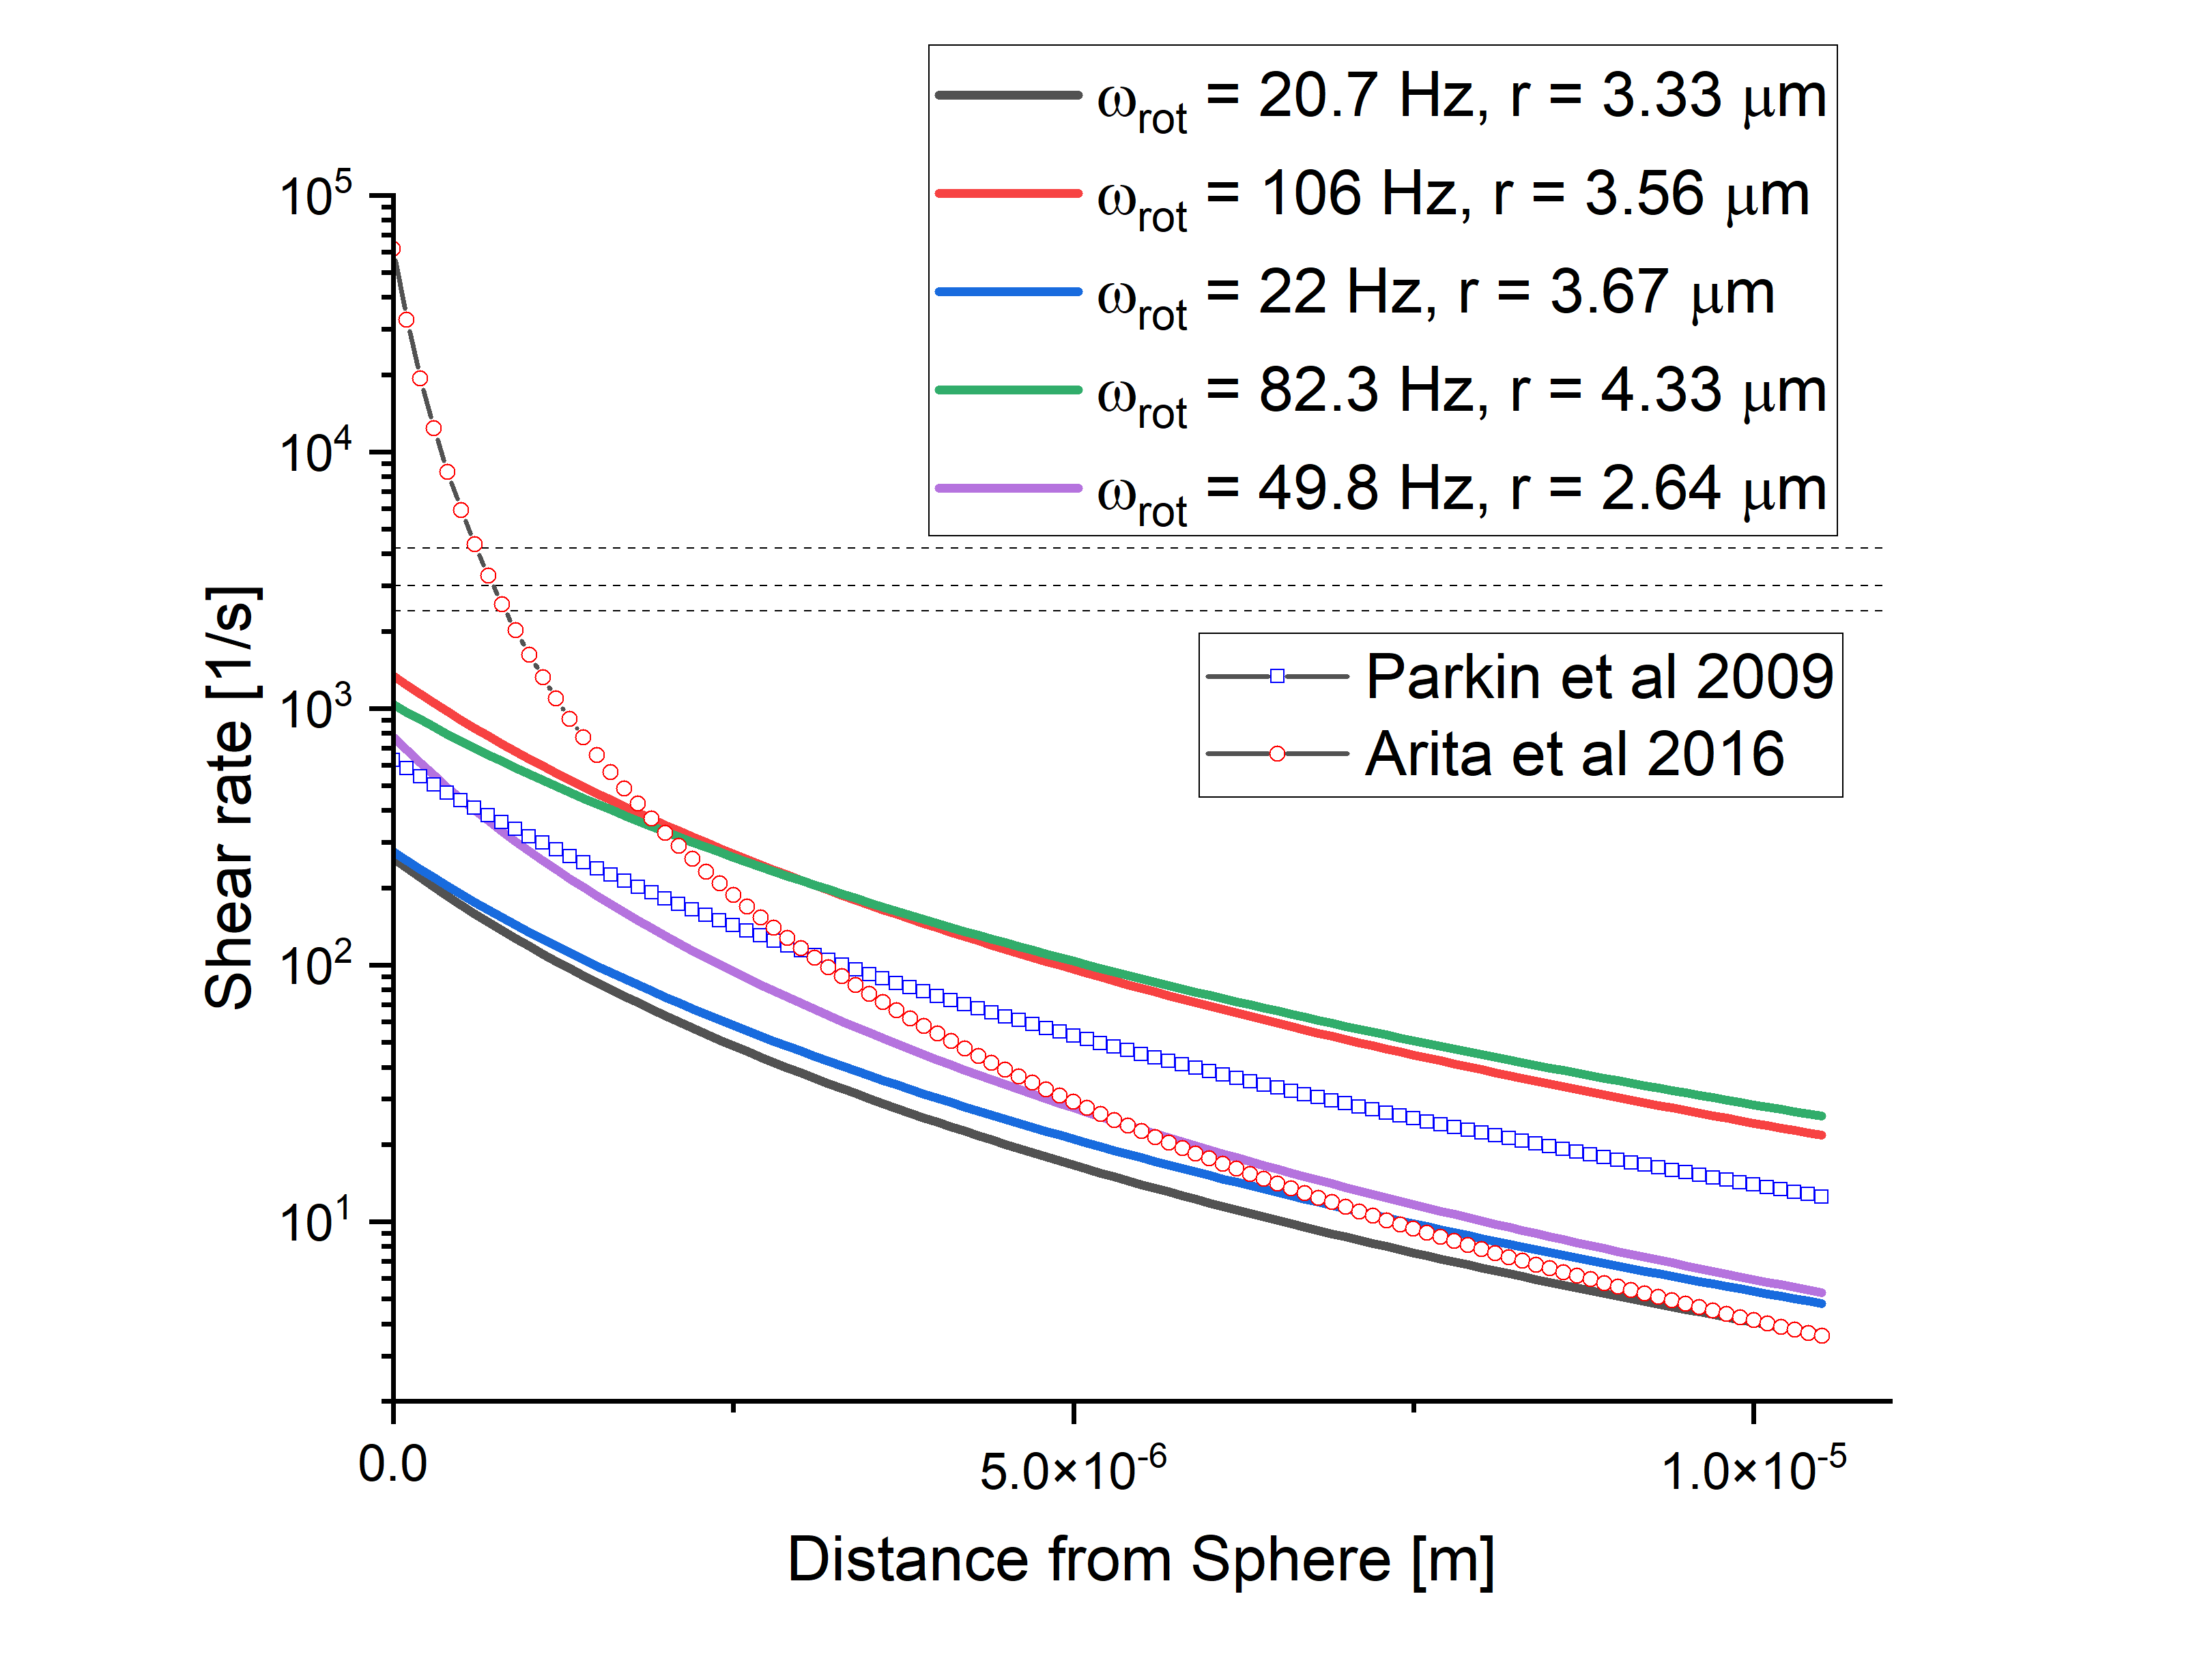
\includegraphics[width=\linewidth]{vaterite_shear_rate.png}
		\subcaption{}
	\end{subfigure}
	\caption{(a) Fluid flow radiating out from the surface of a rotating vaterite sphere. (b) Shear rates computed using Eq.\ref{eq:birefringent_shear}, optimal shear rate is of $3000 s^{-1}$ is indicated by the dotted line. Vaterite radii and rotation frequencies are shown, the laser power was kept constant at 450 mW. Reported rotation rates, and their corresponding fluid flow and shear rates, for vaterite are also plotted alongside lab results.}
\end{figure}

From Fig.\ref{fig:vaterite_shear}~(b) it's clear that the rotational speeds
achieved both in the lab and from experimental literature are well below the 
theoretical maximum shear rate reported by \cite{Debuysschere2023} as you move 
away from the surface of your micro-rotor.

Vaterite samples were synthesised according to \cite{Parkin2009, Bishop2004} 
(see sec.~\ref{sec:vaterite}), and then suspended in a droplet of supersaturated solutions of Glycine and water. After locating a singular microsphere the
vaterite was trapped in a circularly polarised light and brought close
to the droplet edge, after a period of ten minutes if no nucleation event
was observed the particle was released and another particle was trapped. 
Due to the increased viscosity of the supersaturated solution and the 
proximity to the droplet edge, the observed rotation rate 
was rather low or non-existent, the results are tabulated below:

\begin{table}
	\centering
	\caption{Results from rotating vaterite within supersaturated solution. Solubility concentration for Glycine was at $16^\circ$, $C^*=0.2016g/g$}
	\begin{tabular}[width=\textwidth]{|c|c|c|c|}
		\hline
		Super Saturation & Particle radius [$\mu$] & $\omega$ [Hz] & Nucleation [$\checkmark/\times$]\\
		\hline
		\multirow{3}*{1.01} & 2.34 & 20.7 & $\times$ \\
		\cline{2-4} & 5.67 & 23.3 & $\times$ \\
		\cline{2-4} & 3.26 & 15.4 & $\times$ \\
		\hline
		\multirow{3}*{1.14} & 1.89 & 1.23 & $\times$ \\
		\cline{2-4} & 3.75 & 3.54 & $\times$ \\
		\cline{2-4} & 4.35 & 4.86 & $\times$ \\
		\hline
		\multirow{3}*{1.29} & 3.47 & 0.00 & $\times$ \\
		\cline{2-4} & 1.59 & 0.00 & $\times$ \\
		\cline{2-4} & 6.24 & 0.00 & $\times$ \\
		\hline
		\multirow{3}*{1.40} & 6.32 & 0.00 & $\times$ \\
		\cline{2-4} & 3.68 & 0.00 & $\times$ \\
		\cline{2-4} & 5.43 & 0.00 & $\times$ \\
		\hline
		\multirow{3}*{1.49} & 4.76 & $0.00$ & $\times$ \\
		\cline{2-4} & 7.27 & $0.00$ & $\times$ \\
		\cline{2-4} & 1.52 & $0.00$ & $\times$ \\
		\hline
	\end{tabular}
\end{table}


This would explain partly why we could never seen nucleation even in the case where our vaterite could rotate freely. The closest we could trap a microsphere to the droplet edge was in the range of $5-10\mu\ m$, at that distance the fluid flow would be so low that not even using a liquid droplet rotor would achieve the rotational speeds necessary to localise nucleation.

Using a galvano mirror can A particle's motion can be precisely controlled For a simple circular path one can estimate the sphere's speed by the radius of its path and the frequency of its orbit $U = R\omega$; however for a more complex path, such as an elliptical orbit the curve needs to be parametrised. One can describe the position parameter of an ellipse as such:

\begin{align}
	r(u) = \left[acos(2\pi u),bsin(2\pi u), 0 \right]
\end{align}

where a and b are the different characteristic radii of an ellipse, if we assume that u describes time from some initial point we can say $u=t\omega$ where omega is the frequency of orbit. Subbing this in and then taking the partial derivative of position gives:

\begin{align}
	v(t) = \frac{dr(t)}{dt} = \left[-2\pi a\omega \ sin(2\pi t\omega),\ 2\pi b\omega \ cos(2\pi t\omega),0 \right]
\end{align}

In order to compute U we simply take the magnitude of our velocity. For low velocities the fluid flow around the entire sphere can be computed based on the sphere's velocity.

\begin{align}
	u_r(r)=-v(t)cos(\theta)\left(1-\frac{3R}{2r}+\frac{R^3}{2r^3}\right)
\end{align}

Where $\theta$ is the angle from the direction of movement to the point you wish to measure, and $r$ is the radial distance to that point. Again taking the partial derivative we can get the shear rate for a particle moving through the fluid:

\begin{align}
	\dot{\gamma}(r) = \left| \frac{\delta u_r(r)}{\delta r}\right| = v(t)cos(\theta)\left(\frac{3R}{r^2} -\frac{2R^3}{r^4} \right)
\end{align}

Silica beads ($r=1,57 \mu m$) were trapped and moved along an elliptical path
